\chapter{Yukawa Theory: Interacting Spinor and Scalar Fields}
In the previous chapters we have described the Free Dirac Field. We arrived at it from the U(1) invariant Lagrangian for two Weyl spinors, we quantized it, solved its equations of motion in terms of a mode expansion and extracted the creation and annihilation operators. Now we focus on interacting theory of the Dirac Field. We construct its LSZ formula to calculate scattering amplitudes, and find the Dirac Field Propagator and Path Integral to calculate correlation functions. At last, we consider Yukawa theory: the theory of interactions between Dirac Fields and scalar fields.
\section{LSZ reduction formula for fermions}
We consider one-particle states 
\begin{equation}
    \begin{split}
    \ket{p,s,+}&=b^\dagger_s(\vb{p})\ket{0}\\
    \ket{p,s,-}&=d^\dagger_s(\vb{p})\ket{0}
    \end{split}
\end{equation}
where the label $\pm$ in the state kets refers to their U(1) charge eigenvalue : $b$-type particles are electrons with $+1$ U(1) charge and $d$-type are positrons with $-1$ U(1) charge. We consider the Lorentz invariant normalization of one-particle states
\begin{equation}
    \braket{p,s,q}{p^\prime,s^\prime,q^\prime}=(2\pi)^32\omega\delta^3(\vb{p}-\vb{p}^\prime)\delta_{ss^\prime}\delta_{qq^\prime}
\end{equation}
and the mass-shell relation $\omega=\sqrt{\vb{p}^2+m^2}$. We introduce wave-packet creation operators, such as
\begin{equation}
    b^\dagger_1\equiv\int\dd^3 p\,ḱ f_1(\vb{p})b^\dagger_{s_1}(\vb{p})
\end{equation}
creating a particle (electron) with spin $s_1$ spread around 3-momentum $\vb{p}_1$ with a gaussian envelope $f_1(\vb{p})\propto\exp[-(\vb{p}-\vb{p}_1)^2/4\sigma^2]$. The initial state with two particles reads
\begin{equation}
    \ket{i}=b_1^\dagger b_2^\dagger\ket{0}.
\end{equation}
As time goes by, the packets spread and separate. In the infinite past, they correspond to widely separated particle states. As usual, these are considerations in free theory. In the interacting theory, creation operators pick up time dependence, but as long as the field obeys certain conditions, we can take
\begin{equation}
    \ket{i}=\lim _{t\to-\infty}b_1^\dagger(t) b_2^\dagger(t)\ket{0}
\end{equation}
\begin{equation}
    \ket{f}=\lim _{t\to\infty}b_{1^\prime}^\dagger(t) b_{2^\prime}^\dagger(t)\ket{0}
\end{equation}
as initial and final two-particle states, and consder the amplitude $\braket{f}{i}$ for scattering.
With appropriate normalization of $f_i(\vb{p})$ we can make $\braket{f}=\braket{i}=1$. To get the amplitude $\braket{f}{i}=\vev{\,b_{2^\prime}(+\infty)b_{1^\prime}(+\infty)b_1^\dagger(-\infty)b_2^\dagger(-\infty)}$ we consider, as we did for the scalar field, the difference
\begin{equation}
    \begin{aligned}
    b_1^\dagger(-\infty)-b_1^\dagger(+\infty)=&-\int_{-\infty}^{+\infty}\dd t\,\partial_0b_1^\dagger(t)\\
    &=-\int\dd^3 p\, f_1(\vb{p})\int \dd^4 x\,\partial_0\qty(e^{ipx}\Bar{\Psi}(x)\gamma^0u_{s_1}(\vb{p}))\\
    &=-\int\dd^3 p\, f_1(\vb{p})\int \dd^4x\,\Bar{\Psi}(\gamma^0\overleftarrow{\partial}_0-i\overbrace{\gamma^0p^0}^{\gamma^jp^j+m})u_{s_1}(\vb{p})e^{ipx}\\
    &=-\int\dd^3 p\, f_1(\vb{p})\int \dd^4x\,\Bar{\Psi}(\gamma^0\overleftarrow{\partial}_0-\gamma^j\overrightarrow{\partial}_j-im)u_{s_1}(\vb{p})e^{ipx}\\
    &=-\int\dd^3 p\, f_1(\vb{p})\int \dd^4x\,\Bar{\Psi}(\gamma^0\overleftarrow{\partial}_0+\gamma^j\overleftarrow{\partial}_j-im)u_{s_1}(\vb{p})e^{ipx}\\
    &=i\int\dd^3 p\, f_1(\vb{p})\int \dd^4x\,\Bar{\Psi}(i\gamma^0\overleftarrow{\partial}_0+i\gamma^j\overleftarrow{\partial}_j+m)u_{s_1}(\vb{p})e^{ipx}\\
    &=i\int\dd^3 p\, f_1(\vb{p})\int \dd^4x\,\Bar{\Psi}(+i\overleftarrow{\slashed{\partial}}+m)u_{s_1}(\vb{p})e^{ipx}\\
    \end{aligned}
    \label{b1_spinor}
\end{equation}
The first line is the fundamental theorem of calculus; the second comes from (\ref{bdagger_psi}), expressing the creation operator in terms of the Dirac field; the third comes from distributing the derivative, and the over-brace expression indicates that the action of $\gamma^0p^0$ on $u_{s_1}$ equals that of $\gamma^jp^j+m$ on it, according to (\ref{uv}). The fourth line comes from replacing $ip^j$ for the derivative to act on $e^{ipx}$. The fifth comes from realizing that $\Bar{\Psi}\gamma^j\partial_je^{ipx}=\gamma^j\partial_j(\Bar{\Psi} e^{ipx})-(\gamma^j\partial_j\Bar{\Psi})e^{ipx}$ and that the first term is a surface term that can be made to vanish as long as $f_1(\vb{p})$ goes to zero fast enough (this is the role of $f_1(\vb{p})$ in our considerations). The sixth equality comes from factoring out the $i$ and the seventh from recognizing the slashed derivative. Hermitian conjugation gives 
\begin{equation}
    b_1(+\infty)-b_1(-\infty)=i\int\dd^3p\,f_1(\vb{p})\int\dd^4x\,e^{-ipx}\bar{u}_{s_1}(\vb{p})(-i\slashed{\partial}+m)\Psi(x),
    \label{b1}
\end{equation}
And similar considerations lead to
\begin{equation}
    d^\dagger_1(+\infty)-d^\dagger_1(-\infty)=i\int\dd^3p\,f_1(\vb{p})\int\dd^4x\,e^{ipx}\bar{v}_{s_1}(\vb{p})(-i\slashed{\partial}+m)\Psi(x),
    \label{d1dagger}
\end{equation}
\begin{equation}
     d_1(+\infty)-d_1(-\infty)=-i\int\dd^3 p\, f_1(\vb{p})\int \dd^4x\,\Bar{\Psi}(x)(+i\overleftarrow{\slashed{\partial}}+m)v_{s_1}(\vb{p})e^{-ipx}.
     \label{d1}
\end{equation}
Back to the amplitude, we insert a time-ordering symbol
\begin{equation}
    \braket{f}{i}=\vev{\text{T}\,b_{2^\prime}(+\infty)b_{1^\prime}(+\infty)b_1^\dagger(-\infty)b_2^\dagger(-\infty)}
    \label{fi911}
\end{equation}
and take the limit $\sigma\to0$, which makes $f_1(\vb{p})\to\delta^3(\vb{p}-\vb{p}_1)$. Distributing the products using what we found in (\ref{b1_spinor}) and (\ref{b1})
\begin{equation}
\begin{aligned}
\braket{f}{i}&=i^4\int\dd^4x_1\dd^4x_2\dd^4x_{1^\prime}\dd^4x_{2^\prime}e^{ip_1x_{1}}e^{ip_2x_{2}}e^{-ip^\prime_1x_{1^\prime}}e^{-ip^\prime_2x_{2^\prime}}\\
&\qquad\times[\bar{u}_{s_1^\prime}(\vb{p}_1^\prime)(-i\slashed{\partial}_{{1^\prime}}+m)]_{\alpha_1^\prime}[\bar{u}_{s_2^\prime}(\vb{p}_2^\prime)(-i\slashed{\partial}_{{2^\prime}}+m)]_{\alpha_2^\prime}\\
&\qquad\times\vev{\text{T}\,\Psi_{\alpha^\prime_2}(x_{2^\prime})\Psi_{\alpha^\prime_1}(x_{1^\prime})\bar{\Psi}_{\alpha_1}(x_1)\bar{\Psi}_{\alpha_2}(x_2)}
\\&\qquad\times[(i\overleftarrow{\slashed{\partial}}_{1}+m)u_{s_1}(\vb{p}_1)]_{\alpha_1}[(i\overleftarrow{\slashed{\partial}}_{2}+m)u_{s_2}(\vb{p}_2)]_{\alpha_2}
\end{aligned}
\end{equation}
since the time-ordering moves annihilation operators to the right, where they annihilate $\ket{0}$ and creation operators to the left, where they annihilate $\bra{0}$.
This is the amplitude for electron-electron scattering, since both the initial and final states consist of electron states. We can consider different processes by constructing different particle states. Substitution of eqs (\ref{b1_spinor})-(\ref{d1}) into $\braket{f}{i}$, distribution of products and the effect of time-ordering can be obtained with the direct replacements of creation and annihilation operators into $\braket{f}{i}$ in (\ref{fi911})
\begin{equation}
    b^\dagger_s(\vb{p})_{\text{in}}\to i\int\dd^4x\,\bar{\Psi}(x)(i\overleftarrow{\slashed{\partial}}+m)u_s(\vb{p})e^{ipx}
\end{equation}
\begin{equation}
    b_s(\vb{p})_{\text{out}}\to i\int\dd^4x\,e^{-ipx}\bar{u}_s(\vb{p})(-i{\slashed{\partial}}+m)\Psi(x)
\end{equation}
\begin{equation}
    d^\dagger_s(\vb{p})_{\text{in}}\to -i\int\dd^4x\,e^{ipx}\bar{v}_s(\vb{p})(-i{\slashed{\partial}}+m)\Psi(x)
\end{equation}
\begin{equation}
    d_s(\vb{p})_{\text{out}}\to -i\int\dd^4x\,\bar{\Psi}(x)(i\overleftarrow{\slashed{\partial}}+m)v_s(\vb{p})e^{-ipx}
\end{equation}
where ``in" and ``out" refer to $t=-\infty$ and $t=+\infty$ respectively.\\

Now, as for the requirements for validity of the previous considerations,  we need the field in the interacting theory to work comparably to how it does in the free theory. More specifically, we need it to satisfy
\begin{equation}
    \vev{\Psi(x)}=0
\end{equation}
which states Lorentz invariance, since, considering the commutator
\begin{equation}
    \comm{\Psi(0)}{M^{\mu\nu}}=S^{\mu\nu}\Psi(0).
\end{equation}
the Lorentz invariant vacuum states satisfy $M^{\mu\nu}\ket{0}=0$, so the former expression tells that $S^{\mu\nu}\vev{\Psi(0)}=0$. From translation invariance, we need $\vev{\Psi(x)}=0$ so everthing is consistent with Lorentz invariance. Besides this condition, we also need
\begin{equation}
    \bra{p,s,+}\Psi(x)\ket{0}=0
    \label{charge_cond1}
\end{equation}
\begin{equation}
    \bra{p,s,-}\bar{\Psi}(x)\ket{0}=0.
    \label{charge_cond2}
\end{equation}
which comes from the fact that
\begin{equation}
    \comm{\Psi(x)}{Q}=+\Psi(x)
    \label{charge_condition1}
\end{equation}
\begin{equation}
    \comm{Q}{\bar{\Psi}(x)}=+\bar{\Psi}(x)
    \label{charge_condition2}
\end{equation}
which can be verified by recalling that $Q=\int\dd^3 x \bar{\Psi}\gamma^0\Psi$ and by using the field anti-commutation relations (\ref{anticomm_dirac}). Taking the matrix element by multiplying by $\bra{p,s,\pm}$ on the left and by $\ket{0}$ on the right on both sides of (\ref{charge_condition1}) and (\ref{charge_condition2}), bearing in mind that $Q\ket{0}=0$, leads to (\ref{charge_cond1}) and (\ref{charge_cond2}), which state charge conservation. At last, considering the mode expansion (\ref{dirac_mode_expansion}) and the anti-commutation relations (\ref{anticomm_dirac}), we also need 
\begin{equation}
    \bra{p,s,-}\Psi(x)\ket{0}=v_s(\vb{p})e^{-ipx}
\end{equation}
\begin{equation}
    \bra{p,s,+}\bar{\Psi}(x)\ket{0}=\bar{u}_s(\vb{p})e^{-ipx}.
\end{equation}
To meet all these requirements, we can re-scale and shift the Dirac field, so that its equations of motion follow effectively from a rescaled Lagrangian, as, for instance,
\begin{equation}
    \mathcal{L}=iZ\bar{\Psi}\slashed{\partial}\Psi-Z_mm\bar{\Psi}\Psi-\frac{1}{4}Z_gg(\bar{\Psi}\Psi)^2.
\end{equation}
As usual, $Z_mm$ is fixed to correspond to the particle's mass, $Z_g g$ fixed to reproduce a particular scattering cross-section, and $Z$ is fixed by making the field consistent with the conditions we just highlighted.
\section{Free propagator for the Dirac field}
As in the scalar field case, we are interested in the Dirac differential operator Green's function, as a first step toward building more elaborate correlation functions and also to be able to evaluate the free Dirac Field functional integral. We consider Dirac Fields $\Psi(x)$ and $\bar{\Psi}(y)$ and their mode expansion. We define the \textit{Feynman Propagator} for the Dirac Field as
\begin{equation}
    S_{\alpha\beta}(x-y)\equiv i\vev{\text{T}\,\Psi_\alpha(x)\bar{\Psi}_\beta(y)}
\end{equation}
Where $\text{T}$ stands for the \textit{time ordering symbol}, which implements the time ordering of the fields according to
\begin{equation}
    \text{T}\Psi_\alpha(x)\bar{\Psi}_\beta(y)=\theta(x^0-y^0)\Psi_\alpha(x)\bar{\Psi}_\beta(y)-\theta(y^0-x^0)\bar{\Psi}_\beta(y)\Psi_\alpha(x)
\end{equation}
where $\theta(x)$ is the unit step function, defined to be $0$ for $x\leq0$ and $1$ for $x>0$. Note that the minus sign in the second term comes in due to the anticommutation of the fields. Evaluating the vacuum expected value of $\vev{\Psi_\alpha(x)\bar{\Psi}_\beta(y)}$ using the mode expansion (\ref{dirac_mode_expansion}), the first anti-commutation relation of (\ref{coef_anticomm}) and the first relation of (\ref{spin_sum}) for spin sums of products of $u_s(\vb{p)}$ and $\bar{u}_s(\vb{p})$ gives
\begin{equation}
    \vev{\Psi_\alpha(x)\bar{\Psi}_\beta(y)}=\int\widetilde{\dd p}\,e^{ip(x-y)}(-\slashed{p}+m)_{\alpha\beta}.
\end{equation}
Similarly, using barred (\ref{dirac_mode_expansion}), the second anti-commutation relation of \ref{coef_anticomm}) and the second of (\ref{spin_sum}) for spin sums gives 
\begin{equation}
    \vev{\bar{\Psi}_\beta(y)\Psi_\alpha(x)}=\int\widetilde{\dd p}\,e^{-ip(x-y)}(-\slashed{p}-m)_{\alpha\beta}.
\end{equation}
Noting that, for a polynomial function of $p$, say $f(p)$, evaluation of the time integral in the following Fourier transform gives
\begin{equation}
\begin{aligned}
\int\frac{\dd^4p}{(2\pi)^4}\frac{e^{ip(x-y)}f(p)}{p^2+m^2-i\epsilon}&=i\theta(x^0-y^0)\int\widetilde{\dd p}\,e^{ip(x-y)}f(p)\\&\qquad+ i \theta(y^0-x^0)\int\widetilde{\dd p}\,e^{-ip(x-y)}f(-p),
\end{aligned}
\end{equation}
then
\begin{equation}
    \vev{\text{T}\Psi_\alpha(x)\bar{\Psi}_\beta(y)}=\frac{1}{i}\int\frac{\dd^4 p}{(2\pi)^4}\frac{e^{ip(x-y)}(-\slashed{p}+m)_{\alpha\beta}}{p^2+m^2-i\epsilon}.
\end{equation}
So we conclude that the Feynman propagator for the Dirac Field is
\begin{equation}
    S_{\alpha\beta}(x-y)=\int\frac{\dd^4 p}{(2\pi)^4}\frac{e^{ip(x-y)}(-\slashed{p}+m)_{\alpha\beta}}{p^2+m^2-i\epsilon},
    \label{dirac_free_prop}
\end{equation}
which is the Green's function for the Dirac operator
\begin{equation}
\begin{aligned}
    (-i\slashed{\partial}_x+m)_{\alpha\beta}S_{\beta\gamma}(x-y)&=\int\frac{\dd^4 p}{(2\pi)^4}\frac{e^{ip(x-y)}(\slashed{p}+m)_{\alpha\beta}(-\slashed{p}+m)_{\beta\gamma}}{p^2+m^2-i\epsilon}\\
    &=\int\frac{\dd^4 p}{(2\pi)^4}\frac{e^{ip(x-y)}(p^2+m^2)\delta_{\alpha\gamma}}{p^2+m^2-i\epsilon}\\
    &\underbrace{=}_{\epsilon\to0}\quad\delta^4(x-y)\delta_{\alpha\gamma}
\end{aligned}
\end{equation}
similarly, we have
\begin{equation}
    S_{\alpha\beta}(x-y)(+i\overleftarrow{\slashed{\partial}}_y+m)_{\beta\gamma}=\delta^4(x-y)\delta_{\alpha\gamma}.
\end{equation}
At last we note that
\begin{equation}
    \vev{\text{T}\Psi_\alpha(x)\Psi_\beta(y)}=0
\end{equation}
\begin{equation}
    \vev{\text{T}\bar{\Psi}_\alpha(x)\bar{\Psi}_\beta(y)}=0
\end{equation}
since the fields anticomute. 
\section{Path integral for the Dirac field}
To study the functional integral for the Dirac field, we need to define anti-commuting sources $\eta(x)$ and $\bar{\eta}(x)$ so that the following are satisfied
\begin{equation}
    \fdv{\eta(x)}\int\dd^4 y \qty[\bar{\eta}(y)\Psi(y)+\bar{\Psi}(y)\eta(y)]=-\bar{\Psi}(x),
    \label{anticom_source}
\end{equation}
\begin{equation}
    \fdv{\bar{\eta}(x)}\int\dd^4 y \qty[\bar{\eta}(y)\Psi(y)+\bar{\Psi}(y)\eta(y)]={\Psi}(x).
\end{equation}
This way, we consider the free Lagrangian for the Field
\begin{equation*}
    \mathcal{L}_0=-\bar{\Psi}(-i\slashed{\partial}+m)\Psi
\end{equation*}
and add source terms to the action in the functional integral
\begin{equation}
    Z_0(\bar{\eta},\eta)=\int\mathcal{D}\Psi\mathcal{D}\bar{\Psi}\,\exp[i\int\dd^4x(\mathcal{L}_0+\bar{\eta}\Psi+\bar{\Psi}\eta)].
\end{equation}
In analogy with the complex scalar field, we expect this integral to be expressed in terms of the free propagator
\begin{equation}
    Z_0(\bar{\eta},\eta)=\exp[i\int\dd^4x\,\dd^4 y\,\bar{\eta}(x)S(x-y)\eta(y)].
    \label{Z_0_dirac}
\end{equation}
Where $S(x-y)$ is given by (\ref{dirac_free_prop}) (we have omitted the bispinor indices). The choice of normalization is $Z(0,0)=1$, since the vacuum-vacuum amplitude must remain unchanged in the absence of sources.\\

Still in analogy with the complex scalar field, we calculate correlation functions with
\begin{equation}
    \vev{\text{T}\Psi_{\alpha_1}(x_1)\dots\bar{\Psi}_{\beta_1}(y_1)}\dots\equiv\frac{1}{i}\fdv{\bar{\eta}_{\alpha_1}(x_1)}\dots i\fdv{\eta_{\beta_1}(y_1)}\dots Z_0(\bar{\eta},\eta)\eval_{\eta=\bar{\eta}=0}
\end{equation}
Notice the factor $i$ instead of $\frac{1}{i}$ accompanying derivatives with respect to $\eta$ This is because of the anti-commutativity of sources, as (\ref{anticom_source}) shows.
\section{Yukawa theory}
In interacting field theory, we have
\begin{equation}
    Z(\bar{\eta},\eta)\propto\exp[i\int\dd^4x\,\mathcal{L}_1\qty(i\fdv{\eta(x)},\frac{1}{i}\fdv{\bar{\eta}(x)})]Z_0(\bar{\eta},\eta)
\end{equation}
where $\mathcal{L}_1$ is the interaction Lagrangian. We will consider now \textit{Yukawa Theory}: the theory of interaction between the Dirac field and a scalar field. This is the theory of electrons and positrons interacting with scalar particles. The interaction Lagrangian is
\begin{equation}
    \mathcal{L}_1=g\phi\bar{\Psi}\Psi
    \label{yukawa_lagrangian}
\end{equation}
where the Dirac field corresponds to fermions with mass $m$ and the scalar field corresponds to scalars with mass $M$ (we are considering a \textit{real} scalar field). $g$ is a coupling constant. Notice that this Lagrangian is U(1) invariant, so its addition to the free Lagrangian does not break the U(1) invariance the free theory of fermions presents. This means Yukawa theory preserves the U(1) charge and thus the number of electrons minus the number of positrons.\\

Considering the interaction Lagrangian (\ref{yukawa_lagrangian}), the functional integral reads
\begin{equation}
Z(\bar{\eta}, \eta, J) \propto \exp \left[i g \int d^{4} x\left(\frac{1}{i} \frac{\delta}{\delta J(x)}\right)\left(i \frac{\delta}{\delta \eta_{\alpha}(x)}\right)\left(\frac{1}{i} \frac{\delta}{\delta \bar{\eta}_{\alpha}(x)}\right)\right] Z_{0}(\bar{\eta}, \eta, J)
\label{yukawa_Z}
\end{equation}
where the $Z_0$ reads
\begin{equation}
\begin{aligned}
Z_{0}(\bar{\eta}, \eta, J)&= \exp \left[i \int \dd^{4} x\, \dd^{4} y\, \bar{\eta}(x) S(x-y) \eta(y)\right] \\ &\qquad\times
\exp \left[\frac{i}{2} \int \dd^{4} x\, \dd^{4} y\, J(x) \Delta(x-y) J(y)\right].
\end{aligned}
\end{equation}

Series expansion of (\ref{yukawa_Z}) and introduction of Feynman Diagrams again allows us to write
\begin{equation}
    Z(\bar{\eta},\eta,J)=\exp iW(\bar{\eta},\eta,J)
\end{equation}
where $iW(\bar{\eta},\eta,J)$ is the sum of connected diagrams with sources, ignoring tadpoles. \\

In these diagrams, we use dashed lines for scalar propagators $\frac{1}{i}\Delta(x-y)$ and solid lines for fermion propagators $\frac{1}{i}S(x-y)$. The vertex is where two fermion propagators and one scalar propagator meet and has the corresponding factor of $ig\int\dd^4x$. Sources are the blobs at the end of lines and are identified as scalar sources if they rest at the end of scalar lines or as fermion sources if they rest at the end of fermion lines. Since the fermion field accommodates charges we need an arrow rule, just as in the complex scalar field case. Arrows pointing away from the source indicate that such source corresponds to  $i\int\dd^4 x\,\eta(x)$ while  arrows pointing toward a source indicate that such source correspond to $i\int\dd^4x\,\bar{\eta}(x)$. To ensure charge conservation, each vertex must have one arrow pointing toward the vertex, and one arrow pointing away from it. Some diagrams contributing up $g^2$ are shown.
\begin{figure}[h]

    \begin{subfigure}[]{0.2\textwidth}
    \centering
    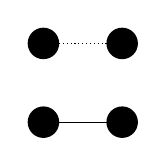
\begin{tikzpicture}
    \fill [black] (0,0) circle (0.2 cm);
    \draw (0,0) -- node {\midarrow} (1,0);
    \fill [black] (1,0) circle (0.2 cm);
    \fill [black] (0,1) circle (0.2 cm);
    \draw (0,1)[densely dotted] --  (1,1);
    \fill [black] (1,1) circle (0.2 cm);
    \end{tikzpicture}
   \caption{$S=2$}
    \end{subfigure}
    ~ 
    \begin{subfigure}[]{0.2\textwidth}
    \centering
    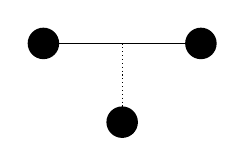
\begin{tikzpicture}
     \fill [black] (0,0) circle (0.2 cm);
    \draw (0,0) -- node {\midarrow} (1,0);
    \draw (1,0) -- node {\midarrow} (2,0);
    \fill [black] (2,0) circle (0.2 cm);
    \draw (1,0)[densely dotted] --  (1,-1);
    \fill [black] (1,-1) circle (0.2 cm);
    \end{tikzpicture}
    \caption{$S=1$}
    \end{subfigure}
    ~ 
    \begin{subfigure}[]{0.3\textwidth}
    \centering
    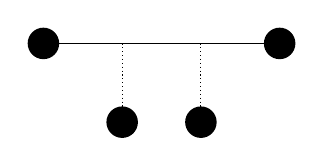
\begin{tikzpicture}
     \fill [black] (0,0) circle (0.2 cm);
    \draw (0,0) -- node {\midarrow} (1,0);
    \draw (1,0) -- node {\midarrow} (2,0);
    \draw (2,0) -- node {\midarrow} (3,0);
    \fill [black] (2,-1) circle (0.2 cm);
    \draw (2,0)[densely dotted] --  (2,-1);
    \fill [black] (3,0) circle (0.2 cm);
    \draw (1,0)[densely dotted] --  (1,-1);
    \fill [black] (1,-1) circle (0.2 cm);
    \end{tikzpicture}
    \caption{$S=1$}
    \end{subfigure}
     ~ 
    \begin{subfigure}[]{0.2\textwidth}
    \centering
    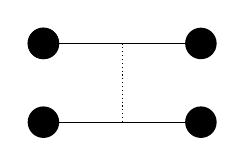
\begin{tikzpicture}
    \fill [black] (0,0) circle (0.2 cm);
    \draw (0,0) -- node {\midarrow} (1,0);
    \draw (1,0) -- node {\midarrow} (2,0);
    \fill [black] (2,0) circle (0.2 cm);
    \draw (1,0)[densely dotted] --  (1,-1);
    \fill [black] (0,0) circle (0.2 cm);
    \draw (0,-1) -- node {\midarrow} (1,-1);
    \draw (1,-1) -- node {\midarrow} (2,-1);
    \fill [black] (2,-1) circle (0.2 cm);
    \fill [black] (0,-1) circle (0.2 cm);
    \end{tikzpicture}
    \caption{$S=2$}
    \end{subfigure}
    \caption{ Diagrams contributing to (\ref{yukawa_Z})}
    \label{yukawa_diag}
\end{figure}
 
\subsection{Scattering amplitude for $e^-\phi\to e^-\phi$}
We prepare initial and final states containing an electron and a scalar, and calculate the amplitude for scattering
\begin{equation}
    \braket{f}{i}=\vev{\text{T}a(\vb{k}^\prime)_{\text{out}}b_{s^\prime}(\vb{p}^\prime)_{\text{out}}b^\dagger_{s}(\vb{p})_{\text{in}}a^\dagger(\vb{k})_{\text{in}}}.
\end{equation}
To this end, we consider (\ref{b1_spinor}) and (\ref{b1}) for $b_{s^\prime}(\vb{p}^\prime)_{\text{out}}$ and $b^\dagger_{s}(\vb{p})_{\text{in}}$, and 
\begin{equation}
    a^\dagger(\vb{k})_{\text{in}}\to i\int\dd^4 z_1 e^{ikz_1}(-\partial^2_{z_1}+M^2)\phi(z_1)
    \label{ain}
\end{equation}
\begin{equation}
    a(\vb{k}^\prime)_{\text{out}}\to i\int\dd^4 z_2 e^{-ik^\prime z_2}(-\partial^2_{z_2}+M^2)\phi(z_2)
    \label{aout}
\end{equation}
So that
\begin{equation}
\begin{aligned}
\braket{f}{i}&=i^4\int\dd^4z_2\,\dd^4x\,\dd^4y\,\dd^4z_1\,e^{-ik^\prime z_2}e^{-ip^\prime x}e^{ipy}e^{ikz_1}(-\partial^2_{z_1}+M^2)(-\partial^2_{z_2}+M^2)\\&\qquad\times \bar{u}_{s^\prime}(\vb{p}^\prime)(-i\slashed{\partial}_x+m)\vev{\text{T}\phi(z_2)\Psi(x)\bar{\Psi}(y)\phi(z_1)}(i\overleftarrow{\slashed{\partial}}_y+m)u_s(\vb{p}).
\end{aligned}
\end{equation}
The fully connected correlation function for such scattering is the sum of connected diagrams with two scalar sources and two fermion sources (Figure \ref{yukawa_diag}-(c)), but with these sources removed
\begin{equation}
\begin{aligned}
\vev{\text{T}\Psi(x)\bar{\Psi}(y)\phi(z_1)\phi(z_2)}&=\frac{1}{i}\fdv{\bar{\eta}(x)}i\fdv{\eta(y)}\frac{1}{i}\fdv{J(z_1)}\frac{1}{i}\fdv{J(z_2)}iW(\bar{\eta},\eta,J)\eval_{\bar{\eta}=\eta=J=0}\\&=
\begin{gathered}
  \begin{tikzpicture}
    \draw (0,0) -- node {\midarrow} (1,0);
    \draw (1,0) -- node {\midarrow} (2,0);
    \draw (2,0) -- node {\midarrow} (3,0);
    \draw (2,0)[densely dotted] --  (2,-1);
    \draw (1,0)[densely dotted] --  (1,-1);
    \node at (-0.2,0.2){$y$};
    \node at (1,0.2){$w_1$};
    \node at (2,0.2){$w_2$};
    \node at (3.2,0.2){$x$};
    \node at (1,-1.2){$z_1$};
    \node at (2,-1.2){$z_2$};
    \end{tikzpicture}
\end{gathered}+
\begin{gathered}
  \begin{tikzpicture}
    \draw (0,0) -- node {\midarrow} (1,0);
    \draw (1,0) -- node {\midarrow} (2,0);
    \draw (2,0) -- node {\midarrow} (3,0);
    \draw (2,0)[densely dotted] --  (2,-1);
    \draw (1,0)[densely dotted] --  (1,-1);
    \node at (-0.2,0.2){$y$};
    \node at (1,0.2){$w_1$};
    \node at (2,0.2){$w_2$};
    \node at (3.2,0.2){$x$};
    \node at (1,-1.2){$z_2$};
    \node at (2,-1.2){$z_1$};
    \end{tikzpicture}
\end{gathered}\\
&=\qty(\frac{1}{i})^5(ig)^2\int\dd^4w_1\,\dd^4w_2\,\\
&\qquad\qquad\qquad\times S(x-w_2)S(w_2-w_1)S(w_1-y)\\&\qquad\qquad\qquad\times\Delta(z_1-w_1)\Delta(z_2-w_2)\\&\qquad\qquad\qquad+(z_1 \leftrightarrow z_2)+\order{g^4}.
\end{aligned}
\end{equation}
Where the scalar fields can be rearranged because they commute with the spinor fields.
Plugging into the LSZ gives
\begin{equation}
    \braket{f}{i}=(2\pi)^4\delta^4(p+k-p^\prime-k^\prime)ig^2\,\bar{u}_{s^{\prime}}\left(\mathbf{p}^{\prime}\right)\left[\frac{-\slashed{p}-\slashed{k}+m}{-s+m^{2}}+\frac{- \slashed{p}+\slashed{k}^{\prime}+m}{-u+m^{2}}\right] u_{s}(\mathbf{p}),
\end{equation}
where  $s=-(p+k)^2$ and $u=-(p-k^\prime)^2$. The $i\epsilon$s were dropped since we have no risk of getting a pole for physically significant values of $s$ and $u$. This result highlights the scattering amplitude for $e^-\phi\to e^-\phi$
\begin{equation}
    i\mathcal{T}_{e^-\phi\to e^-\phi}=ig^2\bar{u}_{s^{\prime}}\left(\mathbf{p}^{\prime}\right)\left[\frac{-\slashed{p}-\slashed{k}+m}{-s+m^{2}}+\frac{- \slashed{p}+\slashed{k}^{\prime}+m}{-u+m^{2}}\right] u_{s}(\mathbf{p}).
    \label{electron_scalar}
\end{equation}
\subsection{Scattering amplitude for $e^+\phi\to e^+\phi$}
For this process, we need to calculate the amplitude
\begin{equation}
    \braket{f}{i}=\vev{\text{T}\,a(\vb{k}^\prime)_{\text{out}}d_{s^\prime}(\vb{p}^\prime)_{\text{out}}d^\dagger_{s}(\vb{p})_{\text{in}}a^\dagger(\vb{k})_{\text{in}}}.
\end{equation}
We use (\ref{d1dagger}) and (\ref{d1}) for $d^\dagger_s(\vb{p})_{\text{in}}$ and $d_{s^\prime}(\vb{p}^\prime)_{\text{out}}$ and (\ref{ain}) and (\ref{aout}) for $a^\dagger(\vb{k})_{\text{in}}$ and $a(\vb{k}^\prime)_{\text{out}}$. This gives us
\begin{equation}
\begin{aligned}
\braket{f}{i}&=i^4\int\dd^4z_2\dd^4x\dd^4y\dd^4z_1e^{-ik^\prime z_2}e^{-ip^\prime y}e^{ipx}e^{ikz_1}(-\partial^2_{z_1}+M^2)(-\partial^2_{z_2}+M^2)\\&\times \bar{v}_{s}(\vb{p})(-i\slashed{\partial}_x+m)\vev{\text{T}\phi(z_2)\bar{\Psi}(y)\Psi(x)\phi(z_1)}(i\overleftarrow{\slashed{\partial}}_y+m)v_{s^\prime}(\vb{p}^\prime)
\end{aligned}
\end{equation}
The fully connected correlation function ends up being equal to that of the previous process, but with an overall minus sign due to the exchange of spinor fields. This has no physical effect since we will be interested in squares of absolute values of $\braket{f}{i}$
\begin{equation}
\begin{aligned}
\vev{\text{T}\bar{\Psi}(y)\Psi(x)\phi(z_1)\phi(z_2)}&=i\fdv{\eta(y)}\frac{1}{i}\fdv{\bar{\eta}(x)}\frac{1}{i}\fdv{J(z_1)}\frac{1}{i}\fdv{J(z_2)}iW(\bar{\eta},\eta,J)\eval_{\bar{\eta}=\eta=J=0}\\
&=-\qty(\frac{1}{i})^5(ig)^2\int\dd^4w_1\,\dd^4w_2\,\\
&\qquad\qquad\qquad\times S(x-w_2)S(w_2-w_1)S(w_1-y)\\&\qquad\qquad\qquad\times\Delta(z_1-w_1)\Delta(z_2-w_2)\\&\qquad\qquad\qquad+(z_1 \leftrightarrow z_2)+\order{g^4}.
\end{aligned}
\end{equation}
Plugging in the LSZ gives
\begin{equation}
    \braket{f}{i}=(2\pi)^4\delta^4(p+k-p^\prime-k^\prime)ig^2\bar{v}_s(\vb{p})\qty[\frac{\slashed{p}+\slashed{k}+m}{-s+m^2}+\frac{\slashed{p}-\slashed{k}^\prime+m}{-u+m^2}]v_{s^\prime}(\vb{p}^\prime)
\end{equation}
meaning we have a scattering amplitude of
\begin{equation}
    i\mathcal{T}_{e^+\phi\to e^+\phi}=ig^2\bar{v}_s(\vb{p})\qty[\frac{\slashed{p}+\slashed{k}+m}{-s+m^2}+\frac{\slashed{p}-\slashed{k}^\prime+m}{-u+m^2}]v_{s^\prime}(\vb{p}^\prime)
    \label{positron_scalar}
\end{equation}
These two scattering amplitudes we calculated  from the LSZ and the correlation functions can be cast directly from momentum-space Feynman Diagrams.
\subsection{Feynman rules for Yukawa theory}
Below are the \textit{Feynman Rules for Yukawa Theory} to find $i\mathcal{T}$ from momentum-space diagrams
\begin{itemize}
    \item Incoming electrons correspond to solid lines with arrows pointing toward the vertex and are labeled with momentum $p_i$;
    \item Outgoing electrons correspond to solid lines with arrows pointing away from the vertex, and are labeled with momentum $p^\prime_i$;
    \item Incoming positrons correspond to solid lines with arrows pointing away from the vertex and are labeled with momentum $-p_i$;
    \item Outgoing positrons correspond to solid lines with arrows pointing toward the vertex and labeled with momentum $-p_i^\prime$
    \item Incoming scalars correspond to dashed lines with arrows pointing toward the vertex and are labeled with momentum $k_i$
    \item Outgoing scalars correspond to dashed lines with arrows pointing away from the vertex and are labeled with momentum $k^\prime_i$;
    \item The vertex is where two solid fermion lines and one dashed scalar line meet. One fermion arrow must point toward the vertex and the other must point away from it. Scalar lines can point in either directions;
    \item With these rules, draw all the topologically inequivalent diagrams-- those that cannot be transformed into others by a deformation of lines-- by joining external lines and adding internal lines if needed;
    \item Think of momentum as a fluid flowing along the arrows and demand its conservation at the vertices. To each internal line, assign a 4-momentum from this conservation requirement;
    \item Incoming or outgoing scalar lines translate to  the factor 1;
    \item Incoming electron lines translate to the factor $u_{s_i}(\vb{p}_i)$;
    \item Outgoing electron lines  translate to $\bar{u}_{s_i^\prime}(\vb{p}^\prime_i)$;
    \item Incoming positron lines translate to $\bar{v}_{s_i}(\vb{p}_i)$;
    \item Outgoing positron lines translate to $v_{s_i^\prime}(\vb{p}_i^\prime)$;
    \item Vertices translate to $ig$;
    \item Internal scalar lines with momentum $k$ translate to $\frac{-i}{k^2+M^2-i\epsilon}$;
    \item Internal fermion lines with momentum $p$ translate to $\frac{-i(-\slashed{p}+m)}{p^2+m^2-i\epsilon}$;
    \item The rule for contraction of spinor indices: locate an external fermion line corresponding either to $\bar{u}$ or $\bar{v}$; go back along that line following the arrows backwards; write the vertices and/or propagators from left-to-right as you encounter them; the last factor should be either $u$ or $v$.
    \item The rule for the sign of a tree-diagram: when drawing tree-diagrams, draw all fermion lines horizontally with a fixed configuration of labels at the endpoints. Next, build the different combinations by switching labels. This will give a permutation of the right endpoints of fermion lines: even permutations give a positive overall sign to the diagram while odd permutations give it a minus sign.
    \item To find $i\mathcal{T}$ translate the diagrams and sum over diagrams 
\end{itemize}
To see the origin of the sign rule, consider the fully connected correlation function
\begin{equation}
\begin{aligned}
\vev{\text{T}\,\Psi(x)\bar{\Psi}(y)\Psi(z)\bar{\Psi}(w)}&=\frac{1}{i}\fdv{\bar{\eta}(x)}i\fdv{\eta(y)}\frac{1}{i}\fdv{\bar{\eta}(z)}i\fdv{\eta(w)}iW(\bar{\eta},\eta,J)\eval_{\bar{\eta}=\eta=J=0}\\
&=\begin{gathered}
  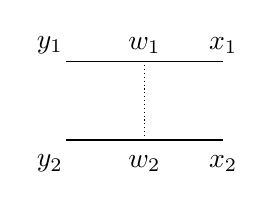
\begin{tikzpicture}
    \draw (0,0) -- node {\midarrow} (1,0);
    \draw (1,0) -- node {\midarrow} (2,0);
    \draw (0,-1) -- node {\midarrow} (1,-1);
    \draw (1,-1) -- node {\midarrow} (2,-1);
    \draw (1,0)[densely dotted] --  (1,-1);
    \node at (-0.2,0.2){$y_1$};
    \node at (1,0.2){$w_1$};
    \node at (2,0.2){$x_1$};
    \node at (1,-1.3){$w_2$};
    \node at (-0.2,-1.3){$y_2$};
    \node at (2,-1.3){$x_2$};
    \end{tikzpicture}
\end{gathered}-
\begin{gathered}
  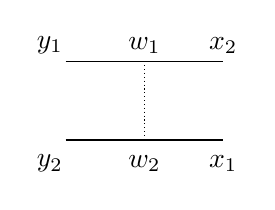
\begin{tikzpicture}
    \draw (0,0) -- node {\midarrow} (1,0);
    \draw (1,0) -- node {\midarrow} (2,0);
    \draw (0,-1) -- node {\midarrow} (1,-1);
    \draw (1,-1) -- node {\midarrow} (2,-1);
    \draw (1,0)[densely dotted] --  (1,-1);
    \node at (-0.2,0.2){$y_1$};
    \node at (1,0.2){$w_1$};
    \node at (2,0.2){$x_2$};
    \node at (1,-1.3){$w_2$};
    \node at (-0.2,-1.3){$y_2$};
    \node at (2,-1.3){$x_1$};
    \end{tikzpicture}
\end{gathered},
\end{aligned}
\end{equation}
that is, this correlation function is the sum of connected diagrams with 4 fermion sources (Figure \ref{yukawa_diag}-(d)) but with those sources removed. The symmetry factor for this diagram is $S=2$ but since the two $\eta$ derivatives and the two $\bar{\eta}$ derivatives can act on the diagram in two different ways each, we have four terms. Of these four, two of them are duplicates of the other two (those shown in the diagram), thus canceling the symmetry factor and leaving $S=1$ for the tree diagrams.  The minus sign comes from the swap of the derivatives to act at the right side, justifying the sign rule.\\

With these Feynman Rules, results (\ref{electron_scalar}) and (\ref{positron_scalar}) can be represented as
\begin{equation}
    i\mathcal{T}_{e^-\phi\to e^-\phi}=
    \begin{gathered}
  \begin{tikzpicture}
    \draw (0,0) -- node {\midarrow} (1,0);
    \draw (1,0) -- node {\midarrow} (2,0);
    \draw (2,0) -- node {\midarrow} (3,0);
    \draw (2,0)[densely dotted] --  (2,-1);
    \draw (1,0)[densely dotted] --  (1,-1);
    \node at (0,0.4){$p$};
    \node at (1.5,0.5){$p+k$};
    \node at (2.8,0.5){$p^\prime$};
    \node at (0.6,-0.5){$k$};
    \node at (2.4,-0.5){$k^\prime$};
    \draw[-triangle 90] (1,-0.5) -- (1,-0.4);
    \draw[-triangle 90] (2,-0.4) -- (2,-0.5);
    \end{tikzpicture}
\end{gathered}+
\begin{gathered}
  \begin{tikzpicture}
    \draw (0,0) -- node {\midarrow} (1,0);
    \draw (1,0) -- node {\midarrow} (2,0);
    \draw (2,0) -- node {\midarrow} (3,0);
    \draw (2,0)[densely dotted] --  (2,-1);
    \draw (1,0)[densely dotted] --  (1,-1);
    \node at (0,0.4){$p$};
    \node at (1.5,0.5){$p-k^\prime$};
    \node at (2.8,0.5){$p^\prime$};
    \node at (0.6,-0.5){$k^\prime$};
    \node at (2.4,-0.5){$k$};
    \draw[-triangle 90] (2,-0.5) -- (2,-0.4);
    \draw[-triangle 90] (1,-0.4) -- (1,-0.5);
    \end{tikzpicture}
\end{gathered}
\end{equation}
\begin{equation}
    i\mathcal{T}_{e^+\phi\to e^+\phi}=
    \begin{gathered}
  \begin{tikzpicture}
    \draw (0,0) -- node {\midarrowleft} (1,0);
    \draw (1,0) -- node {\midarrowleft} (2,0);
    \draw (2,0) -- node {\midarrowleft} (3,0);
    \draw (2,0)[densely dotted] --  (2,-1);
    \draw (1,0)[densely dotted] --  (1,-1);
    \node at (0,0.4){$-p$};
    \node at (1.5,0.5){$-p-k$};
    \node at (2.8,0.5){$-p^\prime$};
    \node at (0.6,-0.5){$k$};
    \node at (2.4,-0.5){$k^\prime$};
    \draw[-triangle 90] (1,-0.5) -- (1,-0.4);
    \draw[-triangle 90] (2,-0.4) -- (2,-0.5);
    \end{tikzpicture}
\end{gathered}+
\begin{gathered}
  \begin{tikzpicture}
    \draw (0,0) -- node {\midarrowleft} (1,0);
    \draw (1,0) -- node {\midarrowleft} (2,0);
    \draw (2,0) -- node {\midarrowleft} (3,0);
    \draw (2,0)[densely dotted] --  (2,-1);
    \draw (1,0)[densely dotted] --  (1,-1);
    \node at (0,0.4){$-p$};
    \node at (1.5,0.5){$-p+k^\prime$};
    \node at (2.8,0.5){$-p^\prime$};
    \node at (0.6,-0.5){$k^\prime$};
    \node at (2.4,-0.5){$k$};
    \draw[-triangle 90] (2,-0.5) -- (2,-0.4);
    \draw[-triangle 90] (1,-0.4) -- (1  ,-0.5);
    \end{tikzpicture}
\end{gathered}
\end{equation}
and scattering amplitudes for other processes can be easily found, as the examples below show
\begin{equation}
\begin{aligned}
 i\mathcal{T}_{e^+e^-\to\phi\phi}&=\begin{gathered}
  \begin{tikzpicture}
    \draw (0,0) -- node {\midarrow} (1,0);
    \draw (1,0)[densely dotted] -- node {\midarrow} (2,0);
    \draw (0,-1) -- node {\midarrowleft} (1,-1);
    \draw (1,-1)[densely dotted] -- node {\midarrow} (2,-1);
    \draw[-triangle 90] (1,-0.4)--(1,-0.5);
    \draw (1,0) --  (1,-1);
    \node at (-0.2,0.2){$p_1$};
    \node at (2,0.2){$k_1^\prime$};
    \node at (2,-0.5){$p_1-k_1^\prime$};
    \node at (-0.2,-1.3){$-p_2$};
    \node at (2,-1.3){$k_2^\prime$};
    \end{tikzpicture}
\end{gathered}+
\begin{gathered}
  \begin{tikzpicture}
    \draw (0,0) -- node {\midarrow} (1,0);
    \draw (1,0)[densely dotted] -- node {\midarrow} (2,0);
    \draw (0,-1) -- node {\midarrowleft} (1,-1);
    \draw (1,-1)[densely dotted] -- node {\midarrow} (2,-1);
    \draw[-triangle 90] (1,-0.4)--(1,-0.5);
    \draw (1,0) --  (1,-1);
    \node at (-0.2,0.2){$p_1$};
    \node at (2,0.2){$k_2^\prime$};
    \node at (2,-0.5){$p_1-k_2^\prime$};
    \node at (-0.2,-1.3){$-p_2$};
    \node at (2,-1.3){$k_1^\prime$};
    \end{tikzpicture}
\end{gathered}\\
&=ig^2\bar{v}_{s_2}(\vb{p}_2)\qty[\frac{-\slashed{p}_1+\slashed{k}^\prime_1+m}{-t+m^2}+\frac{-\slashed{p}_1+\slashed{k}^\prime_2+m}{-u+m^2}]u_{s_1}(\vb{p}_1),
\end{aligned}
\end{equation}
where $t=-(p_1-k_1^\prime)^2$ and $u=-(p_1-k_2^\prime)^2$.
\begin{equation}
\begin{aligned}
 i\mathcal{T}_{e^-e^-\to e^-e^-}&=\begin{gathered}
  \begin{tikzpicture}
    \draw (0,0) -- node {\midarrow} (1,0);
    \draw (1,0) -- node {\midarrow} (2,0);
    \draw (0,-1) -- node {\midarrow} (1,-1);
    \draw (1,-1) -- node {\midarrow} (2,-1);
    \draw[-triangle 90] (1,-0.4)--(1,-0.5);
    \draw (1,0)[densely dotted] --  (1,-1);
    \node at (-0.2,0.2){$p_1$};
    \node at (2.2,0.3){$p_1^\prime$};
    \node at (2,-0.5){$p_1-p_1^\prime$};
    \node at (-0.2,-1.2){$p_2$};
    \node at (2.2,-1.2){$p_2^\prime$};
    \end{tikzpicture}
\end{gathered}-
\begin{gathered}
  \begin{tikzpicture}
    \draw (0,0) -- node {\midarrow} (1,0);
    \draw (1,0) -- node {\midarrow} (2,0);
    \draw (0,-1) -- node {\midarrow} (1,-1);
    \draw (1,-1) -- node {\midarrow} (2,-1);
    \draw[-triangle 90] (1,-0.4)--(1,-0.5);
    \draw (1,0)[densely dotted] --  (1,-1);
    \node at (-0.2,0.2){$p_1$};
    \node at (2.2,0.3){$p_2^\prime$};
    \node at (2,-0.5){$p_1-p_2^\prime$};
    \node at (-0.2,-1.2){$p_2$};
    \node at (2.2,-1.2){$p_1^\prime$};
    \end{tikzpicture}
\end{gathered}\\
    &=ig^2\qty[\frac{\bar{u}_{s^\prime_1}(\vb{p}_1^\prime)u_{s_1}(\vb{p}_1)\bar{u}_{s^\prime_2}(\vb{p}_2^\prime)u_{s_2}(\vb{p}_2)}{-t+M^2}-\frac{\bar{u}_{s^\prime_2}(\vb{p}_2^\prime)u_{s_1}(\vb{p}_1)\bar{u}_{s^\prime_1}(\vb{p}_1^\prime)u_{s_2}(\vb{p}_2)}{-u+M^2}],
\end{aligned}
\end{equation}
\begin{equation}
\begin{aligned}
 i\mathcal{T}_{e^+e^+\to e^+e^+}&=\begin{gathered}
  \begin{tikzpicture}
    \draw (0,0) -- node {\midarrowleft} (1,0);
    \draw (1,0) -- node {\midarrowleft} (2,0);
    \draw (0,-1) -- node {\midarrowleft} (1,-1);
    \draw (1,-1) -- node {\midarrowleft} (2,-1);
    \draw[-triangle 90] (1,-0.4)--(1,-0.5);
    \draw (1,0)[densely dotted] --  (1,-1);
    \node at (-0.2,0.2){$-p_1$};
    \node at (2.2,0.3){$-p_1^\prime$};
    \node at (2,-0.5){$p_1-p_1^\prime$};
    \node at (-0.2,-1.2){$-p_2$};
    \node at (2.2,-1.2){$-p_2^\prime$};
    \end{tikzpicture}
\end{gathered}-
\begin{gathered}
  \begin{tikzpicture}
    \draw (0,0) -- node {\midarrowleft} (1,0);
    \draw (1,0) -- node {\midarrowleft} (2,0);
    \draw (0,-1) -- node {\midarrowleft} (1,-1);
    \draw (1,-1) -- node {\midarrowleft} (2,-1);
    \draw[-triangle 90] (1,-0.4)--(1,-0.5);
    \draw (1,0)[densely dotted] --  (1,-1);
    \node at (-0.2,0.2){$-p_1$};
    \node at (2.2,0.3){$-p_2^\prime$};
    \node at (2,-0.5){$p_1-p_2^\prime$};
    \node at (-0.2,-1.2){$-p_2$};
    \node at (2.2,-1.2){$-p_1^\prime$};
    \end{tikzpicture}
\end{gathered}\\
    &=ig^2\qty[\frac{\bar{v}_{s_1}(\vb{p}_1)v_{s^\prime_1}(\vb{p}_1^\prime)\bar{v}_{s_2}(\vb{p}_2)v_{s^\prime_2}(\vb{p}_2^\prime)}{-t+M^2}-\frac{\bar{v}_{s_1}(\vb{p}_1)v_{s^\prime_2}(\vb{p}_2^\prime)\bar{v}_{s_2}(\vb{p}_2)v_{s^\prime_1}(\vb{p}_1^\prime)}{-u+M^2}],
\end{aligned}
\end{equation}
\begin{equation}
\begin{aligned}
 i\mathcal{T}_{e^+e^-\to e^+e^-}&=\begin{gathered}
  \begin{tikzpicture}
    \draw (0,0) -- node {\midarrow} (1,0);
    \draw (1,0) -- node {\midarrow} (2,0);
    \draw (0,-1) -- node {\midarrowleft} (1,-1);
    \draw (1,-1) -- node {\midarrowleft} (2,-1);
    \draw[-triangle 90] (1,-0.4)--(1,-0.5);
    \draw (1,0)[densely dotted] --  (1,-1);
    \node at (-0.2,0.25){$p_1$};
    \node at (2.2,0.3){$p_1^\prime$};
    \node at (2,-0.5){$p_1-p_1^\prime$};
    \node at (-0.2,-1.2){$-p_2$};
    \node at (2.2,-1.2){$-p_2^\prime$};
    \end{tikzpicture}
\end{gathered}-
\begin{gathered}
  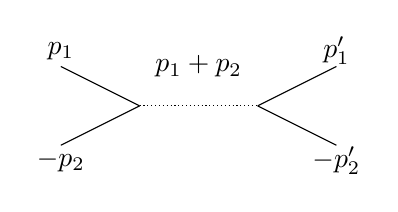
\begin{tikzpicture}
    \draw[densely dotted] (0,0) -- node{\midarrow} (1.5,0);
    \node at (0.75,0.5){$p_1+p_2$};
    \draw (-1,0.5) -- node{\midarrow} (0,0);
    \draw (-1,-0.5) -- node{\midarrowleft} (0,0);
    \draw (2.5,0.5) -- node{\midarrow} (1.5,0);
    \draw (2.5,-0.5) -- node{\midarrowleft} (1.5,0);
    \node at (-1,0.7) {$p_1$};
    \node at (-1,-0.7) {$-p_2$};
    \node at (2.5,0.7) {$p_1^\prime$};
    \node at (2.5,-0.7) {$-p_2^\prime$};
    
    \end{tikzpicture}
\end{gathered}\\
    &=ig^2\qty[\frac{\bar{u}_{s^\prime_1}(\vb{p}_1^\prime)u_{s_1}(\vb{p}_1)\bar{v}_{s_2}(\vb{p}_2)v_{s^\prime_2}(\vb{p}_2^\prime)}{-t+M^2}-\frac{\bar{v}_{s_2}(\vb{p}_2)u_{s_1}(\vb{p}_1)\bar{u}_{s^\prime_1}(\vb{p}_1^\prime)v_{s^\prime_2}(\vb{p}_2^\prime)}{-s+M^2}],
\end{aligned}
\end{equation}
where, in the three cases, $s=-(p_1+p_2)^2$, $t=-(p_1-p_1^\prime)^2$ and $u=-(p_1-p_2^\prime)^2$.